%! Author = TiagoRG
%! GitHub = https://github.com/TiagoRG

\chapter{Detalhes Experimentais Relevantes}
\label{ch:detalhes-experimentais-relevantes}
{
%%%
% Conteúdo da introdução aqui

\section{Parte A}
\label{sec:detalhes-experimentais-relevantes-parte1}

\subsection{Material}
\label{subsec:detalhes-experimentais-relevantes-parte1-material}

\begin{enumerate}
    \item Lançador de projéteis
    \item Suporte para o lançador de projéteis
    \item Sensor de movimento
    \item Sensor de movimento
    \item Sistema de controlo dos sensores
    \item Fita-métrica
    \item Bola metálica
\end{enumerate}

\begin{figure}[h]
    \center
    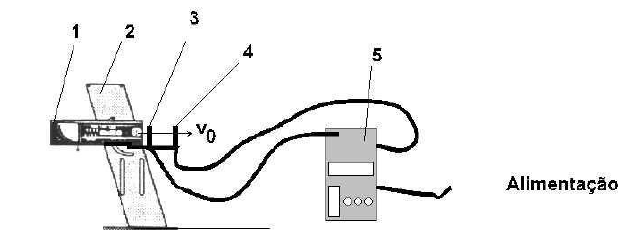
\includegraphics[width=0.8\textwidth]{images/montagem-experimental-parte1}\label{fig:montagem-experimental-parte1}
\end{figure}

\subsection{Procedimento}
\label{subsec:detalhes-experimentais-relevantes-parte1-procedimento}

Antes de iniciar qualquer procedimento experimental é necessário certificar que o lançador de projéteis está devidamente montado e que o sistema de controlo dos sensores está ligado e a funcionar corretamente.

\begin{enumerate}
    \item Preparar a montagem experimental como ilustrado na figura \ref{fig:montagem-experimental-parte1};
    \item Medir a distância entre os sensores de movimento;
    \item Carregar o lançador de projéteis com a bola metálica na posição de tiro curto (SHORT RANGE);
    \item Colocar o sistema de controlo dos sensores na posição de TWO GATES e carregar em START/STOP;
    \item Disparar o projétil e registar o valor de tempo obtidos;
    \item Efetuar 3 disparos e registar as respetivas medições.
\end{enumerate}

\pagebreak

\section{Parte B}
\label{sec:detalhes-experimentais-relevantes-parte2}

\subsection{Material}
\label{subsec:detalhes-experimentais-relevantes-parte2-material}

\begin{enumerate}
    \item Lançador de projéteis
    \item Suporte para o lançador de projéteis
    \item Alvo
    \item Fita-métrica
    \item Bola metálica
\end{enumerate}

\begin{figure}[h]
    \center
    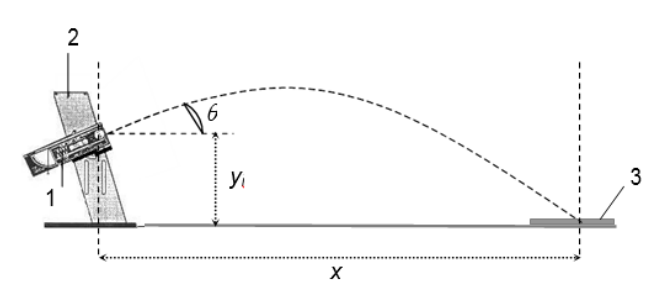
\includegraphics[width=0.8\textwidth]{images/montagem-experimental-parte2}\label{fig:montagem-experimental-parte2}
\end{figure}

\subsection{Procedimento}
\label{subsec:detalhes-experimentais-relevantes-parte2-procedimento}

Antes de efetuar os lançamentos, é necessário verificar rigorosamente o ângulo de lançamento e fixar devidamente o alvo de modo a evitar imprecisões relacionadas com o mesmo.

\begin{enumerate}
    \item Preparar a montagem experimental como ilustrado na figura \ref{fig:montagem-experimental-parte2};
    \item Colocar o alvo a uma distância tal que a esfera caia sobre a sua superfície;
    \item Carregar o lançador de projéteis com a bola na posição de tiro curto (SHORT RANGE);
    \item Medir a altura de lançamento do projétil;
    \item Disparar o projétil e registar o alcance obtido;
    \item Efetuar 3 disparos e registar as respetivas medições para cada valor de ângulo (sendo esses ângulos: 34º, 38º, 40º e 43º).
\end{enumerate}

\pagebreak

\section{Parte C}
\label{sec:detalhes-experimentais-relevantes-parte3}

\subsection{Material}
\label{subsec:detalhes-experimentais-relevantes-parte3-material}

\begin{enumerate}
    \item Suporte para o lançador de projéteis
    \item Lançador de projéteis
    \item Bola metálica
    \item Pêndulo balístico
    \item Balança
    \item Fita-métrica
\end{enumerate}

\begin{figure}[h]
    \center
    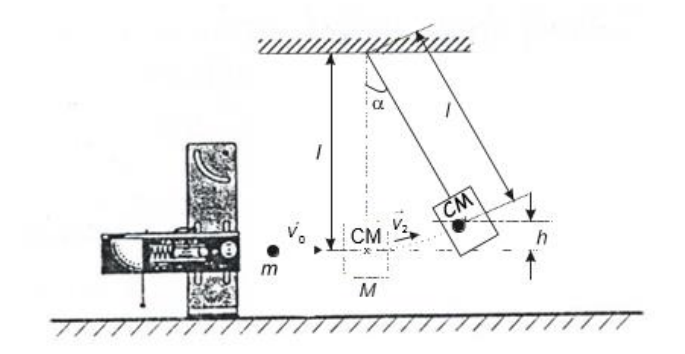
\includegraphics[width=0.8\textwidth]{images/montagem-experimental-parte3}\label{fig:montagem-experimental-parte3}
\end{figure}

\subsection{Procedimento}
\label{subsec:detalhes-experimentais-relevantes-parte3-procedimento}


\begin{enumerate}
    \item Preparar a montagem experimental como ilustrado na figura \ref{fig:montagem-experimental-parte3};
    \item Medir as massas do projétil e do pêndulo balístico;
    \item Medir o comprimento do pêndulo;
    \item Carregar o lançador de projéteis com a bola na posição de tiro curto (SHORT RANGE);
    \item Disparar o projétil e registar o ângulo máximo descrito pelo pêndulo;
    \item Efetuar 5 disparos e registar as respetivas medições.
\end{enumerate}

%%%
}
